\chapter{Fire Plumes, Ceiling Jets, and Device Activation}

\section{Flame Height}

Flame height is recorded by visual observations, photographs, or video footage.  Videos from the NIST/NRC test series and photographs from the VTT Large Hall Test Series were used to estimate flame height.  It is difficult to precisely measure the average flame height, but the photos and videos allow one to make estimates relative to a known burner diameter for the tests.

\subsubsection{VTT Large Hall Test Series}

The height of the visible flame in  photographs has been estimated to be between 2.4 and 3 pan diameters (3.8 m to 4.8 m).  From the CFAST calculations, the estimated flame height is 4.3 m.

\subsubsection{NIST/NRC Test Series}

CFAST estimates the peak flame height to be 2.8 m, consistent with the roughly 3 m flame height observed through the doorway during the test.  The test series was not designed to record accurate measurements of flame height.

\subsubsection{NIST/Navy High Bay Hangar Test Series}

For the 9 Iceland tests, CFAST predicts flame height within 25~\% of the experimentally reported values, with the largest relative differences for the smaller heat release rate fires. Uncertainty in the flame height measurements for the experiments was reported to be $\pm$ 0.5 m, approaching 30~\% of the experimental values for the lower heat release rate fires.

\section{Plume Temperature}

As with the ceiling jet, CFAST includes a specific plume temperature model based on the model of Alpert and Heskestad~\cite{Alpert:SFPE} to account for presence of higher gas temperatures near a target located at the centerline of the fire plume. The correlation has been subjected to validation efforts by \cite{Valid:Davis_Plumes} and shown to provide predictions within about 30 \% of a wide range of experimental results \cite{Valid:Davis_Plumes}. In the model, this increased temperature has the effect of increasing the convective heat transfer to the target. Only two of the six test series (VTT and FM/SNL) included measurements of plume centerline temperature.

Figure \ref{fig:Plume_Temp_Scatter} shows a comparison of predicted and measured values for plume temperature. Appendix B provides individual graphs of model and experimental values. All of the comparisons are to the surrounding gas temperature predicted by CFAST. Comparisons to the target surface temperature or target center temperature would be expected to have a smaller relative difference since all the predictions of surrounding gas temperature are higher than experimental measurements. Following is a summary of the predictions in the two test series.
\label{Plume Temperature}

\begin{figure}
\begin{center}
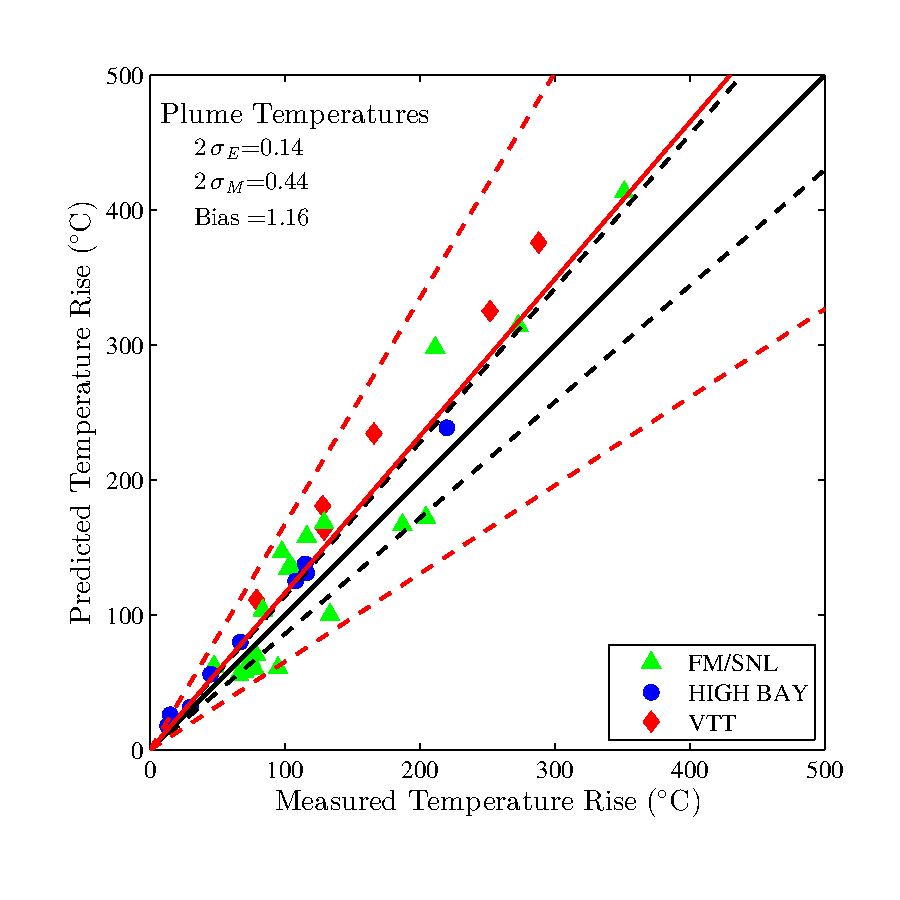
\includegraphics[width=4.0in]{SCRIPT_FIGURES/ScatterPlots/Plume_Temperature}
\end{center}
\caption{Comparison of Measured and Predicted Plume Centerline Temperature.} \label{fig:Plume_Temp_Scatter}
\end{figure}


\section{Ceiling Jets}

CFAST includes an algorithm to account for the presence of the higher gas temperatures near the ceiling surfaces in compartments involved in a fire.  In the model, this increased temperature has the effect of increasing the convective heat transfer to ceiling surfaces.  The temperature and velocity of the ceiling jet are also available from the model by placing a heat detector at the specified location.  The ceiling jet algorithm is based on the model of Alpert and Heskestad~\cite{Alpert:SFPE}, with details described in the CFAST Technical Reference Guide \cite{CFAST_Tech_Guide_7}.  The algorithm predicts gas temperature and velocity under a flat, unconstrained ceiling above a fire source.  Only two of the six test series (NIST/NRC and FM/SNL) involved relatively large flat ceilings.

Figure \ref{fig:Ceiling_Jet_Scatter} shows a comparison of predicted and measured values for ceiling jet temperature. Appendix B provides individual graphs of model and experimental values. Following is a summary of the accuracy assessment for the ceiling jet predictions.
\label{Ceiling Jet Temperature}

\begin{figure}
\begin{center}
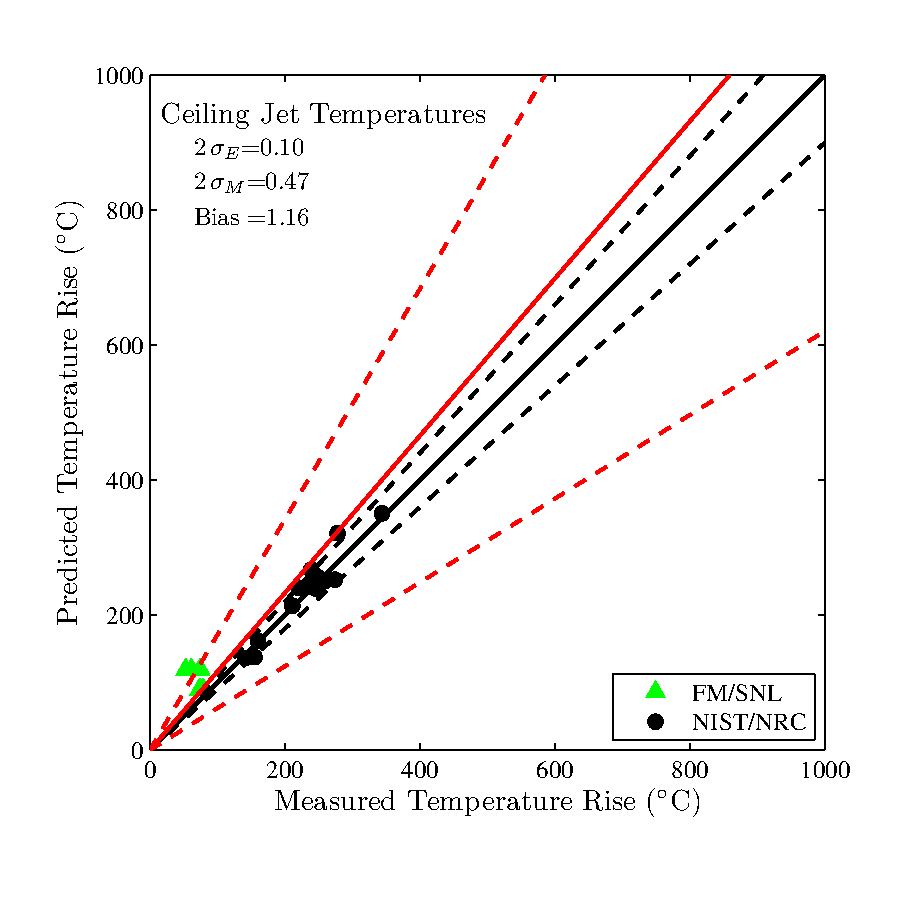
\includegraphics[width=4.0in]{SCRIPT_FIGURES/ScatterPlots/Ceiling_Jet_Temperature}
\end{center}
\caption{Comparison of Measured and Predicted Ceiling Jet Temperature.} \label{fig:Ceiling_Jet_Scatter}
\end{figure}

\section{Device Activation}

Smoke detector, heat detector, and sprinkler activations are all treated similarly in CFAST.  Device activation is modeled using temperatures and velocities from the ceiling jet.  For rooms without a fire (which do not have a ceiling jet), the upper layer temperature (and a default velocity of 0.1 m/s) is used.  Devices are described with a characteristic activation temperature and response time index (RTI). The RTI a measure of the sensor's sensitivity to temperature change (thermal inertia). For heat detectors and sprinklers, the activation temperature and RTI values are part of the device specification. For smoke detectors, a temperature rise of 10~\degc and RTI of 5~(m s)$^{1/2}$ were used, consistent with values in NUREG 1805 \cite{NRCNUREG1805}. With these inputs, the characteristic detector temperature is modeled using the differential equation \cite{Heskestad:1976}

\be \frac{dT_L}{dt} = \frac{\sqrt{v(t)}}{RTI} \brackets{T_g(t) - T_L(t)} \; , \; T_L(0) = T_g(0)  \ee

where $T_L$ and $T_g$ are the link and gas temperatures, $v$ is the gas velocity, and $RTI$.

Figure \ref{fig:Activation_Scatter} shows a comparison of predicted and measured values for activation times. Appendix B provides individual graphs of model and experimental values.
\label{Smoke Detector Activation Time}
\label{Sprinkler Activation Time}

\begin{figure}{t}
\begin{center}
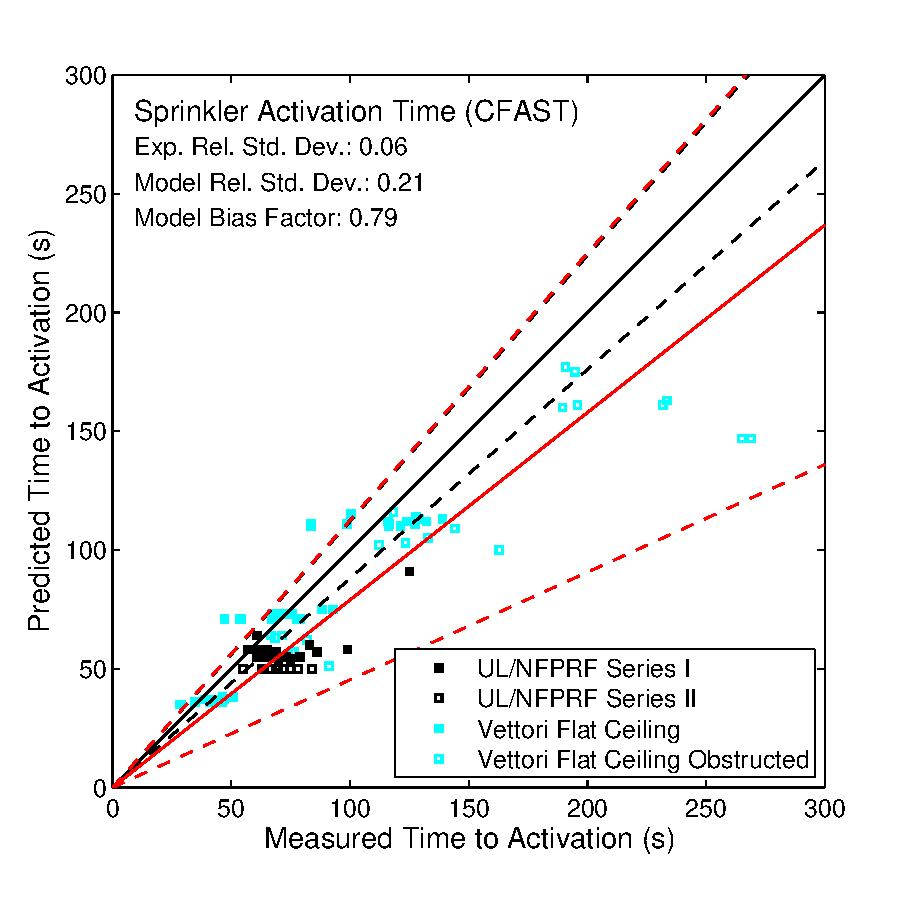
\includegraphics[width=4.0in]{SCRIPT_FIGURES/ScatterPlots/Sprinkler_Activation_Time}  \\
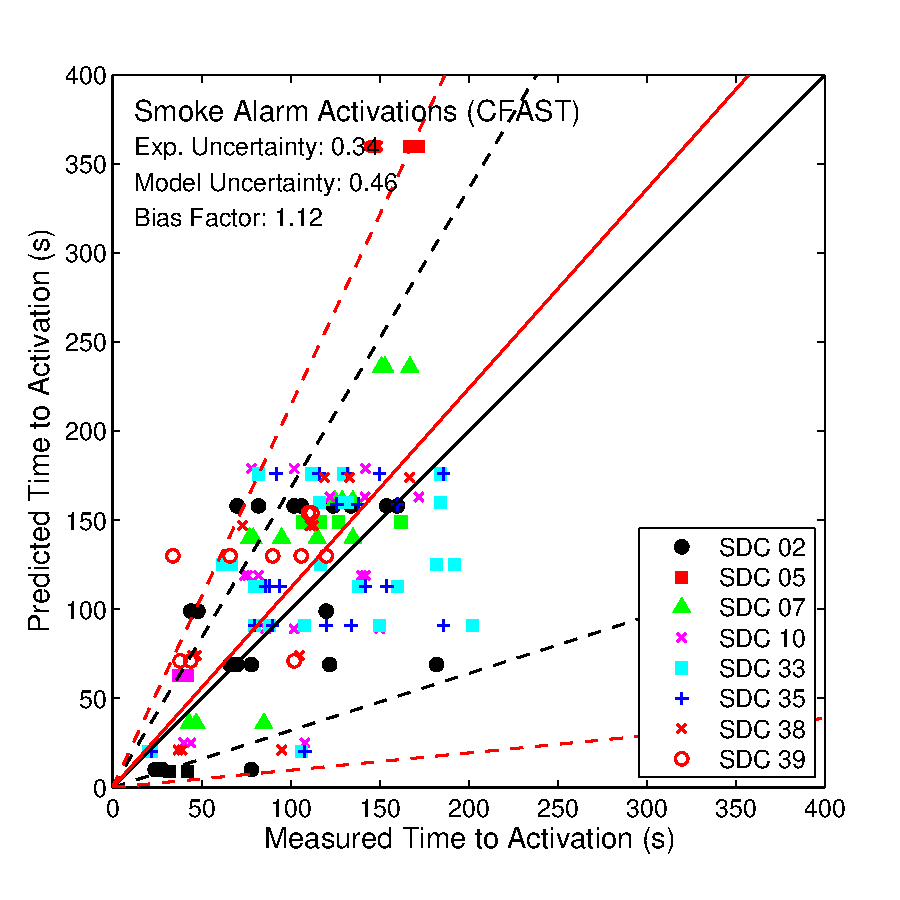
\includegraphics[width=4.0in]{SCRIPT_FIGURES/ScatterPlots/Smoke_Alarm_Activation_Time}
\end{center}
\caption{Comparison of Measured and Predicted Ceiling Jet Temperature.} \label{fig:Activation_Scatter}
\end{figure}





